%\ifdefined\fullcompile \else
\ifdefined\compileall \else
\ifdefined\compiletype
	\documentclass[handout]{beamer}
\else
	\documentclass{beamer}
	\def\compiletype{livebeamer}
\fi

\usepackage{templates/beamerthemekitwide}

\usepackage[utf8]{inputenc}
\usepackage[T1]{fontenc}
\usepackage[ngerman]{babel}
\usepackage{listings}
\usepackage{hyperref}
\usepackage{graphicx}

\usepackage{amsmath}
\usepackage{amsthm}
\usepackage{amssymb}
\usepackage{polynom}

\usepackage{ifthen}
\usepackage{adjustbox} % for \adjincludegraphics

\newcommand{\markBlue}[1]{\textcolor{kit-blue100}{#1}}
\newcommand{\markGreen}[1]{\textcolor{kit-green100}{#1}}

\newcommand{\pitem}{\pause\item}
\newcommand{\p}{\pause}

% -- MATH MACROS
\newcommand{\thistheoremname}{}
\newcommand{\G}{\mathbb{Z}}
\newcommand{\B}{\mathbb{B}}
\newcommand{\R}{\mathbb{R}}
\newcommand{\N}{\mathbb{N}}
\newcommand{\Q}{\mathbb{Q}}
\newcommand{\C}{\mathbb{C}}
\newcommand{\Z}{\mathbb{Z}}
\newcommand{\F}{\mathbb{F}}
\newcommand{\mi}{\mathrm{i}}
\renewcommand{\epsilon}{\varepsilon}


\newenvironment<>{taskblock}[1]{%
	\setbeamercolor{block title}{fg=kit-orange15,bg=kit-orange100}
	\setbeamercolor{block body}{fg=black,bg=kit-orange30}%
	\begin{block}#2{#1}}{\end{block}}

\setbeamertemplate{enumerate items}[default]

% Aussagenlogik Symbole
\newcommand{\W}{w}
\renewcommand{\F}{f}

% Kodierung
\newcommand{\frepr}{\textbf{repr}}
\newcommand{\fRepr}{\textbf{Repr}}
\newcommand{\fZkpl}{\textbf{Zkpl}}
\newcommand{\fbin}{\textbf{bin}}
\newcommand{\fdiv}{\textbf{ div }}
\newcommand{\fmod}{\textbf{ mod }}

\title[Grundbegriffe der Informatik]{Grundbegriffe der Informatik\\Tutorium 33}
\subtitle{}
\author{Lukas Bach, lukas.bach@student.kit.edu}
\date{\tutdate}

\institute{}

\titlelogo{lukasbach}

\titleimage{bg}
%\titleimage{bg-advent}


\ifthenelse{\equal{\compiletype}{livebeamer}}
	{
		\def\livebeamermode{1}
	}{}

\ifthenelse{\equal{\compiletype}{print}}
	{
		\def\printmode{1}
	}{}

\setbeamercovered{invisible}

%\usepackage[citestyle=authoryear,bibstyle=numeric,hyperref,backend=biber]{biblatex}
%\addbibresource{templates/example.bib}
%\bibhang1em

\begin{document}
	
\selectlanguage{ngerman}


%title page
\begin{frame}
	\titlepage
\end{frame}

%table of contents
\ifdefined\printmode
	\ifdefined\compileall \else
	\begin{frame}{Gliederung}
		\tableofcontents
	\end{frame}
\fi\fi

\fi
%\fi

% content
\section{Organisatiorisches}

\begin{frame}{Termine}
	\begin{itemize}
		\pause
		\item Vorlesung und Übung
		\pause
			\begin{itemize}
				\item Mittwoch 9:45 - 11:15 Vorlesung
				\item Freitag 9:45 - 11:15 abwechselnd Vorlesung und Übung
			\end{itemize}
		
		\pause
		\item Tutorium
		\pause
			\begin{itemize}
				\item Donnerstags, 14:00 - 15:30
				\item 50.34 Informatikbau, -107
			\end{itemize}
		
		\pause
		\item Übungsblätter
		\pause
		\begin{itemize}
			\item Alle zwei Wochen
			\item Ausgabe Mittwochs, Abgabe Donnerstags bis 16:00 zwei Wochen drauf %TODO
		\end{itemize}
	\end{itemize}
\end{frame}

\begin{frame}{Übungsschein}
	\begin{itemize}
		\pause
		\item min. 50\% aller Punkte auf Übungsblättern richtig\pause
		\item Rückgabe im Tutorium\pause
		\item Bestehen ist \emph{keine} Voraussetzung für die Klausur\pause , \emph{aber} fürs Modul!\pause
		\item Gemeinsames Abgeben, Abschreiben verboten\pause
		\item Übungsblätter und später auch Musterlösungen im ILIAS
	\end{itemize}
\end{frame}

\begin{frame}{Tutorium}
	\begin{itemize}
		\item Alle Tutorienfolien auf:\pause
	\end{itemize}
	
	\begin{center}
		\url{http://gbi.lukasbach.com}
	\end{center}
	\pause
	
	\begin{itemize}
		\item Bei Fragen: lukas.bach@student.kit.edu\pause
		\item Keine Anwesenheitspflicht\pause
		\item Möglichkeit andere Tutorien zu besuchen
	\end{itemize}
\end{frame}


\section{Signale und Nachrichten}

\begin{frame}{Signale und Nachrichten}
	\begin{itemize}
		\pause\item Objekt: \markBlue{101}
		\begin{itemize}
			\pause\item Eins null eins \pause oder 101 als Zahl \pause oder 5 in binär \pause oder zwei merkwürdige Striche mit einem Kreis dazwischen?
			\pause\item Vom Kontext abhängig.
			\pause\item Zunächst einfach ein konkretes Objekt.
		\end{itemize}
	\end{itemize}
\end{frame}

\begin{frame}{Signale und Nachrichten}	
	\begin{itemize}
		\pause\item Signal
		\begin{itemize}
			\pause\item Physikalische Veränderung
			\pause\item Lässt sich verschieden interpretieren.
			\pause\item Beispiele:
			\begin{itemize}
				\pause\item Notfallalarm in Serverraum\\
				\pause 
\includegraphics[width=.1\linewidth]{images/alarm.jpg}\\
				\pause\item Für Besucher nur schönes Leuchten
				\pause\item Für Security die Information, zu kommen
				\pause\item Für Techniker die Information, Ausrüstung zu holen
			\end{itemize}
		\end{itemize}
		
		\pause\item Nachricht\pause : Objekt wie oben, das von Signal unabhängig ist
		\begin{itemize}
			\pause\item Roter Notfallalarm ist ein anderes Signal als ein blauer Notfallalarm\pause , aber vielleicht dieselbe Nachricht.
		\end{itemize}
	\end{itemize}
\end{frame}

\begin{frame}{Signale und Nachrichten}
	\begin{itemize}
		\pause\item Der interessante Teil: \pause Informationen
		\pause\item Bedeutung einer Nachricht
		\pause\item Der vorher fehlende Kontext.
		\pause\item Im obigen Beispiel:
		\begin{itemize}
			\pause\item Rote Alarmleuchte ist ein Signal \pause (blaue Signalleuchte in Raum nebendran vielleicht auch)
			\pause\item ``Alarm'': Nachricht
			\pause\item Information: \pause Security soll herkommen\pause , Techniker sollen das Werkzeug bereit halten\pause , Besucher sollten Platz machen.
		\end{itemize}
	\end{itemize}
\end{frame}

\section{Mengen}


\begin{frame}{Mengen}
	\begin{itemize}
		\pause\item Erster wirklich wichtiger Teil.
	\end{itemize}
\end{frame}

\begin{frame}{Mengen}
	Zeichnung
\end{frame}

\begin{frame}{Mengen}
	\begin{block}{Definition: Mengen}
		\pause
		``Unter einer Menge \pause verstehen wir jede
		Zusammenfassung \pause von bestimmten \pause
		wohlunterschiedenen \pause Objekten \pause unserer
		Anschauung oder unseres Denkens \pause (welche die
		Elemente dieser Menge genannt werden) \pause zu einem
		Ganzen.''
	\end{block}
	
	%TODO was ist eine definition
	
	\begin{itemize}
		\pitem Beispiel:\pause $\{a, b, c, d\}$ \pause $ =: A$ \pause $\{a, c, 4\} =: B, \{10, 11\} =: C$
		\pitem Das Objekt $c$ ist in $A$ enthalten\pause : $c \in A$\pause , $c \in B$\pause , $c \notin C$
		\pitem Reihenfolge gleich\pause : $\{a, b\} = \{b, a\}$
		\pitem Elemente doppelt? \pause $\{a, a, b, a\} = \{a, b\}$
	\end{itemize}
\end{frame}

\begin{frame}{Mehr über Mengen}
	\begin{itemize}
		\pitem Kardinalität \pause oder Größe\pause : Die Anzahl der Elemente der Menge
		\begin{itemize}
			\pitem $A := \{a, b, c\}$\pause . $|A| = 3$
			\pitem $B := \{c, d\}$\pause . $|B| = 2$
			\pitem Was ist $|\{1, 2, 3, 2\}|$? \pause $3$!
			\pitem Was ist $|\{\}|?$ \pause $0$
		\end{itemize}
	\end{itemize}
	
	\pause
	
	\begin{block}{Leere Menge}
		Die Menge, die nichts enthält, nennen wir die leere Menge\pause , und schreiben sie als $\{\}$ oder $\emptyset$.
	\end{block}
	
	\pause
	
	Was ist $|\{\{\}\}|$? \pause 1! \pause $\{\emptyset\}$ enthält eine leere Menge, die selbst ein Element ist.
\end{frame}


\begin{frame}{Mehr über Mengen}
	Zeichnung
\end{frame}

\begin{frame}{Mehr über Mengen}
	\pause Seien $A := \{a, b, c\}, B:= \{b, c\}, C:= \{c, b\}, D := \{b, c, d\}$.
	
	\begin{itemize}
		\pitem Teilmenge\pause : $A \subseteq B$\pause , also $A$ ist Teilmenge von $B$ \pause genau dann, wenn alle Elemente aus $A$ auch in $B$ sind.
		\pitem Echte Teilmenge\pause : $A \subset B$ \pause genau dann, wenn $A \subseteq B$ \pause \emph{und} $A \neq B$.
		\begin{itemize}
			\pitem Beispiele: \pause $B \subseteq A$\pause , sogar $B \subset A$.\\ \pause $C \subseteq B$ \pause und $B \subseteq C$\pause , aber $C \not\subset B$ und $B \not\subset C$.
		\end{itemize}
		\pitem Schnittmenge\pause : $A \cap B$ \pause $ = \{b, c\}$.\pause \\ $A \cap B$ enthält \emph{genau} die Elemente, die in $A$ \emph{und} in $B$ sind.%TODO erkläre "genau", siehe LA. Wieso übrigens kein := ?
		\pitem Vereinigungsmenge\pause : $A \cup D$ \pause $ = \{a, b, c, d\}$.\pause \\ $A \cup B$ enthält \emph{genau} die Elemente, die in $A$ \emph{oder} in $B$ sind.
		\pitem Mengendifferenz: \pause $A \setminus B$ \pause $ = \{a\}$\pause , also alle Elemente in $A$, die nicht in $B$ sind.
		\pitem Komplementärmenge: \pause $\bar{A}$ \pause enthält alle Elemente des \emph{Universums}, die nicht in $A$ sind. \pause Angenommen, Universum = Lateinisches Alphabet: \pause $\bar{A} = \{d, e, f, g, \dots, y, z\}$
	\end{itemize}
\end{frame}

\begin{frame}{Potenzmenge}
	\pause
	
	\begin{block}{Potenzmenge}
		Die Potenzmenge \pause $2^M$ \pause einer Menge $M$ \pause enthält genau alle Mengen, die Teilmenge von $M$ sind.	
	\end{block}
	
	\pause
	
	Was bedeutet das allgemein?
	
	\begin{itemize}
		\pitem $M \in 2^M$
		\pitem $\emptyset \in 2^M$
		\pitem Konkretes Beispiel: \pause Was ist $2^M$ mit $M = \{0, 1\}$?
		\begin{itemize}
			\pitem Natürlich $\emptyset \in 2^M$ und $\{0, 1\} \in 2^M$.
			\pitem $\{0\} \in 2^M$ \pause und $\{1\} \in 2^M$.
			\pitem Weitere? \pause Nein, diese vier Mengen sind alle möglichen Teilmengen.
			\pitem $\Rightarrow$ $2^M = \{\{\}, \{0\}, \{1\}, \{0, 1\}\}$.
		\end{itemize}
	\end{itemize}
\end{frame}

\begin{frame}{Potenzmenge}
	$M = \{0, 1\}$\pause , $2^M = \{\{\}, \{0\}, \{1\}, \{0, 1\}\}$.\pause
	
	Was ist $2^{2^M}$?
	
	\begin{itemize}
		\pitem Also $2^{\{\{\}, \{0\}, \{1\}, \{0, 1\}\}}$.
		\pitem Natürlich $\emptyset \in 2^M$ und $2^M = \{\{\}, \{0\}, \{1\}, \{0, 1\}\} \in 2^{2^M}$.
	\end{itemize}
	
	\pause
	
	$2^{2^M} \pause
	= 
	\{  $\\$\pause\quad
	\{\},$\\$\pause\quad
	\{\{\}\}, 
	\{\{0\}\}, 
	\{\{1\}\},
	\{\{0, 1\}\}, $\\$\pause\quad
	\{\{\}, \{0\}\}, 
	\{\{\}, \{1\}\}, 
	\{\{\}, \{0, 1\}\}, 
	\{\{0\}, \{1\}\}, $\\$\qquad
	\{\{0\}, \{0, 1\}\}, 
	\{\{1\}, \{0, 1\}, $\\$\pause\quad
	\{\{\}, \{0\}, \{1\}\}, 
	\{\{\}, \{0\}, \{0, 1\}\}, 
	\{\{\}, \{1\}, \{0, 1\}\}, 
	\{\{0\}, \{1\}, \{0, 1\}\}, $\\$\pause\quad
	\{\{\}, \{0\}, \{1\}, \{0, 1\}\} $\\$
	\}
	$
\end{frame}

\section{Alphabete}
\begin{frame}{Alphabete}
	
	\pause
	
	\begin{block}{Alphabet}
		Ein Alphabet ist eine \emph{endliche}, \emph{nichtleere} Menge von Zeichen.
	\end{block}
	
	\pause
	
	Was davon sind Alphabete? \pause $\{d, 34, \pi, \%\}$\pause , $\{a, b, c, \dots, y, z\}$\pause , $\emptyset$\pause , $\N$.
	
	\begin{itemize}
		\pitem $\{d, 34, \pi, \%\}$ und $\{a, b, c, \dots, y, z\}$ sind Alphabete.
		\pitem $\emptyset$ ist leer und damit kein Alphabet.
		\pitem $\N = \{1, 2, 3, \dots\}$ enthält alle natürlichen Zahlen und ist damit nicht endlich, also kein Alphabet.
		\pitem $\{0, 1\}$ ist das Alphabet, das alle Binärzahlen enthält.
		\pitem $\{\cdot, +, -, /\} =: R$ ist ein Alphabet von Rechenzeichen.\pause $R \cup \{0, 1, \dots, 9\}$ ist ein Alphabet, das ein Taschenrechner als Eingabealphabet benutzen könnte.
	\end{itemize}
\end{frame}

\section{Relationen und Abbildungen}
\begin{frame}{Paare und Tupel}
	\pause
	\begin{block}{Paar}
		Ein Paar ist eine geordnete Menge \pause der Kardinalität 2.
	\end{block}
	\pause
	Schreibweise mit runden Klammern ().
	\begin{itemize}
		\pitem Beispiel: $(a, 4)$\pause $\neq (4, a)$
		\pitem Beispiel für eine Menge aus Tupeln: $\{(``Age Of Empires'', ``Strategie''),$ $(``Battlefield'', ``Shooter''),$ $(``Serious Sam'', ```Shooter'')\}$
	\end{itemize}
\end{frame}

\begin{frame}{Tupel}
	\pause
	\begin{block}{Tupel}
		Ein Tupel ist eine geordnete Menge. \pause Konkret ist ein $n$-Tupel ein Tupel der Kardinalität $n$.
	\end{block}
	\pause
	Also wie ein Paar, nur mit beliebiger Kardinalität. \pause Ein Paar ist spezifisch ein 2-Tupel.\pause
	
	Beispiel: $(4tb, 512gb, 128gb, 4mb)$ \pause $\neq (512gb, 4mb, 4tb, 128gb)$.
\end{frame}

\begin{frame}{Kartesisches Produkt}
	Zwei Mengen: $A := \{a, b, c\}$ \pause und $B := \{1, 2, 3\}$. \pause
	
	Wir wollen alle Tupel \pause mit erstem Element aus $A$ \pause und zweiten Element aus $B$.\pause
	
	$\{
	\quad (a, 1), (a, 2), (a, 3), 
	\qquad (b, 1), (b, 2), (b, 3), 
	\qquad (c, 1), (c, 2), (c, 3)\quad
	\}$ \pause $ = A \times B$
	
	\pause
	
	\begin{block}{Kreuzprodukt von zwei Mengen}
		Zu zwei Mengen $A$ und $B$ ist das Kreuzprodukt definiert als Menge aller Paare $(a, b)$ mit $a \in A$ und $b \in B$.
	\end{block}
\end{frame}

\begin{frame}{Kreuzprodukt}
	\begin{block}{Kreuzprodukt von zwei Mengen}
	Zu zwei Mengen $A$ und $B$ ist das Kreuzprodukt $A \times B$ definiert als Menge aller Paare $(a, b)$ mit $a \in A$ und $b \in B$.
	\end{block}
	
	\begin{block}{Kreuzprodukt von n Mengen}
		Zu $n$ Mengen $M_1$, $M_2$, \dots, $M_n$ \pause ist das Kreuzprodukt $M_1 \times M_2 \times \cdots \times M_n$ \pause definiert als Menge aller $n$-Tupel $(e_1, e_2, \dots, e_n)$ \pause mit $e_1 \in M_1$, $e_2 \in M_2$, \dots, $e_n \in M_n$.
	\end{block}\pause
	
	\begin{block}{Mengenpotenz}
		$\underbrace{A \times A \times \cdots \times A}_{n \times mal} = A^n$.
	\end{block}
\end{frame}

\begin{frame}{Kreuzprodukt: Beispiele}
	\begin{block}{Kreuzprodukt von zwei Mengen}
		Zu zwei Mengen $A$ und $B$ ist das Kreuzprodukt $A \times B$ definiert als Menge aller Paare $(a, b)$ mit $a \in A$ und $b \in B$.
	\end{block}
	\pause
	
	$A := \{a, b\}, B := \{1, 2\}$. \pause $A \times B$ \pause $ = \{(a, 1), (a, 2), (b, 1), (b, 2)\}$.
\end{frame}

\begin{frame}{Kreuzprodukt: Beispiele}
	
	\begin{block}{Kreuzprodukt von n Mengen}
		Zu $n$ Mengen $M_1$, $M_2$, \dots, $M_n$ \pause ist das Kreuzprodukt $M_1 \times M_2 \times \cdots \times M_n$ \pause definiert als Menge aller $n$-Tupel $(e_1, e_2, \dots, e_n)$ \pause mit $e_1 \in M_1$, $e_2 \in M_2$, \dots, $e_n \in M_n$.
	\end{block}\pause
	
	$A := \{a, b\}, B := \{1, 2\}, C:= \{\omega\}$. $A \times B \times C$ \pause $ = \{(a, 1, \omega), (a, 2, \omega), (b, 1, \omega), (b, 2, \omega) \}$.
	
\end{frame}

\begin{frame}{Kreuzprodukt: Beispiele}
	
	\begin{block}{Mengenpotenz}
		$\underbrace{A \times A \times \cdots \times A}_{n mal} = A^n$.
	\end{block}\pause
	
	\begin{itemize}
		\item $A := \{a, b\}$. \pause $A^2$ \pause $ = \{(a, b), (b, a), (a, a), (b, b)\}$ \pause $A^3 = \{(a, a, a), (a, a, b), (a, b, b), \dots\}$.
		\pitem $A$ beliebige Menge. \pause $A^0$? \pause $ = \emptyset$ 
		\pitem Achtung! $2^M \neq M^2$. \pause Potenzmengen nicht mit Mengenpotenz verwechseln!
	\end{itemize}
	
\end{frame}

\begin{frame}{Relation}
	\pause
	
	\begin{block}{Binäre Relation}
		Eine binäre Relation auf zwei Mengen $A$ und $B$ ist eine Menge $R \subseteq A \times B$.
	\end{block}\pause
	
	\begin{itemize}
		\item Für die Mengen $M_{Spiele} = \{``Battlefield'', ``AgeOfEmpires'', ``SeriousSam''\}$, $M_{Genre} = \{``Shooter'', ``Strategie''\}$ sind folgendes mögliche Relationen:
		\begin{itemize}
			\pitem $\{(``Age Of Empires'', ``Strategie''),$ $(``Battlefield'', ``Shooter''),$ $(``Serious Sam'', ```Shooter'')\}$
			\pitem $\{(``Age Of Empires'', ``Strategie''), (``Age Of Empires'', ``Shooter'')$
			\pitem $\emptyset$
		\end{itemize}
		\pitem ``Kleinergleichrelation'' auf $M = \{1, 2, 3\}$\pause : $R_\leq = \{(1, 1), (1, 2), (1, 3), (2, 2), (2, 3), (3, 3)\}$ \pause $\in M \times M$
	\end{itemize}
\end{frame}


\begin{frame}{Relation}
	\begin{block}{Binäre Relation}
		Eine binäre Relation auf zwei Mengen $A$ und $B$ ist eine Menge $R \subseteq A \times B$.
	\end{block}\pause
	
	\begin{block}{Ternäre Relation}
		Eine ternäre Relation auf drei Mengen $A$, $B$ und $C$ ist eine Menge $R \subseteq A \times B \times C$.
	\end{block}\pause
	
	\begin{block}{n-äre Relation}
		Eine $n$-äre Relation auf $n$ Mengen $M_1$, $M_2$ ... $M_n$ ist eine Menge $R \subseteq M_1 \times M_2 \times \cdots \times M_n$.
	\end{block}
\end{frame}

\begin{frame}{Linkstotalität}
	\begin{block}{Linkstotale Relation}
		Eine Relation $R \subseteq A \times B$ heißt linkstotal\pause , wenn für jedes $a \in A$ ein $b \in B$ existiert mit $(a,b) \in R$.
	\end{block}\pause
	
	Die linke Seite der Relation ist also ``total'' aufgefüllt.\pause
	
	\begin{center}
		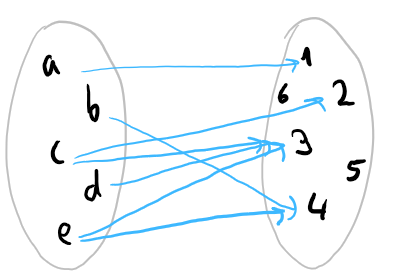
\includegraphics[width=.5\linewidth]{images/mengen_linkstotal.png}
	\end{center}
\end{frame}

\begin{frame}{Rechtstotalität}
	\begin{block}{Rechtstotale Relation}
		Eine Relation $R \subseteq A \times B$ heißt rechtstotal\pause , wenn für jedes $b \in B$ ein $a \in A$ existiert mit $(a,b) \in R$.
	\end{block}\pause
	
	Die rechte Seite der Relation ist also ``total'' aufgefüllt.\pause
	
	\markGreen{Wenn die Relation zusätzlich eine Abbildung ist, heißt diese dann} \markBlue{surjektiv}.\pause
	
	\begin{center}
		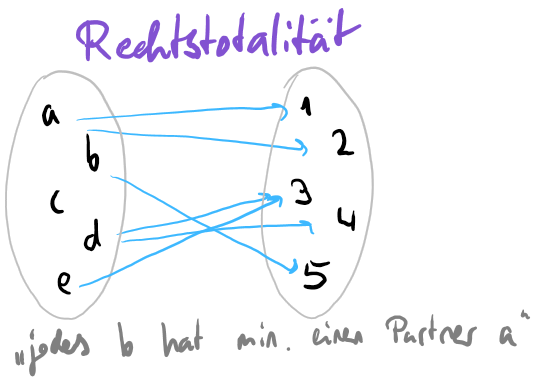
\includegraphics[width=.5\linewidth]{images/mengen_rechtstotal.png}
	\end{center}
\end{frame}

\begin{frame}{Linkseindeutigkeit}
	\begin{block}{Linkseindeutige Relation}
		Eine Relation $R \subseteq A \times B$ heißt linkseindeutig\pause , wenn für zwei beliebige Elemente $(a, \alpha) \in R, (b, \beta) \in R$ aus der Relation $R$ gilt: \pause wenn $a \neq b$, dann gilt auch $\alpha \neq \beta$. 
	\end{block}\pause
	
	Also: Keine zwei Elemente der linken Seite der Relation haben dasselbe rechte Element.\pause
	
	Angenommen, $a \neq b$ und $\alpha = \beta$. \pause $\Rightarrow$ offenbar nicht linkseindeutig.\pause
	
	\markGreen{Wenn die Relation zusätzlich eine Abbildung ist, heißt diese dann} \markBlue{injektiv}.\pause
	
	\begin{center}
		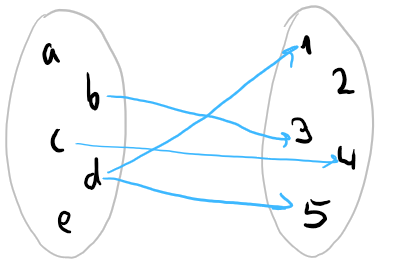
\includegraphics[width=.4\linewidth]{images/mengen_linkseindeutig.png}
	\end{center}
\end{frame}

\begin{frame}{Rechtseindeutig}
	\begin{block}{Rechtseindeutige Relation}
		Eine Relation $R \subseteq A \times B$ heißt rechtseindeutig\pause , wenn für zwei beliebige Elemente $(a, \alpha) \in R, (b, \beta) \in R$ aus der Relation $R$ gilt: \pause wenn $\alpha \neq \beta$, dann gilt auch $a \neq b$. 
	\end{block}\pause
	
	Also: Keine zwei Elemente der rechten Seite der Relation haben dasselbe linke Element.\pause
	
	\begin{center}
		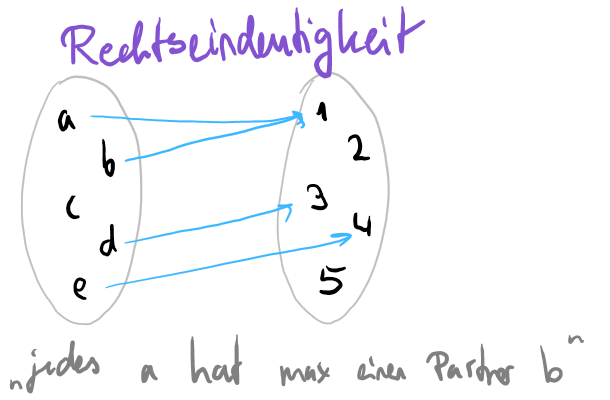
\includegraphics[width=.5\linewidth]{images/mengen_rechtseindeutig.png}
	\end{center}
\end{frame}

\ifdefined\printmode
\begin{frame}{Eigenschaften von Relationen}
	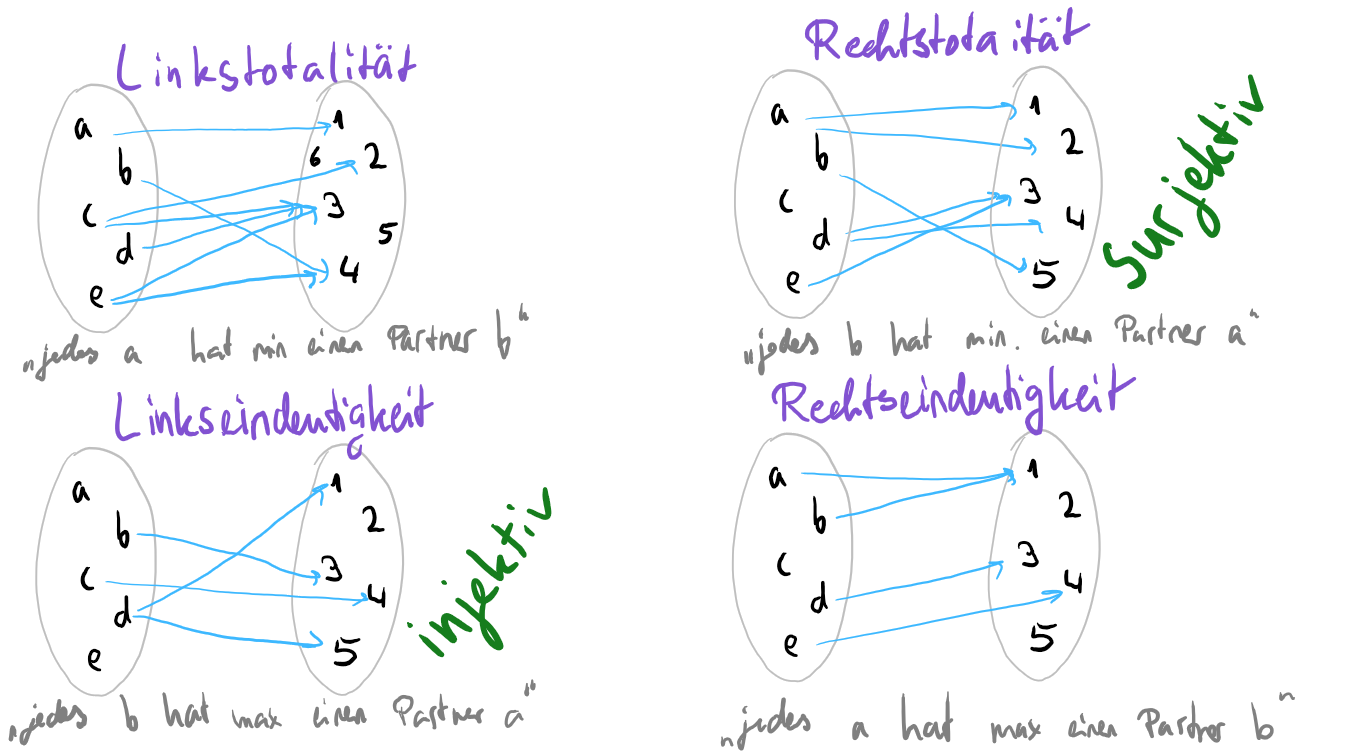
\includegraphics[width=\linewidth]{images/mengen_alle.png}
\end{frame}
\fi

\begin{frame}{Abbildung}
	\pause
	\begin{block}{Abbildung}
		Eine Relation $R$ heißt eine Abbildung, wenn sie linkstotal \emph{und} rechtseindeutig sind.
	\end{block}\pause
	
	\begin{itemize}
		\item Injektive Funktion: \pause \markGreen{linkstotal}, \markGreen{rechtseindeutig}, \markBlue{linkseindeutig}
		\pitem Surjektive Funktion: \pause \markGreen{linkstotal}, \markGreen{rechtseindeutig}, \markBlue{rechtstotal}
	\end{itemize}
	
	\pause
	
	\begin{block}{Bijektivität}
		Eine Relation heißt bijektiv, wenn sie injektiv und surjektiv ist.
	\end{block}
	
	\pause
	
	Damit ist sie \markGreen{linkstotal} und \markGreen{rechtseindeutig} (weil es eine Abbildung ist) und \markBlue{linkseindeutig} (injektiv) und \markBlue{rechtstotal} (surjektiv).
	
	\pause Tolle Eigenschaft: \pause Für jedes Element $(a, b) \in R$ der bijektiven Relation $R$ ist \emph{jedem} $a$ \emph{genau ein} $b$ zugeordnet. 
	
\end{frame}

\begin{frame}{Abbildungen Schreibweise}
	Seien $A = B = \R$, $f \subseteq A \times B$. \pause Wir suchen Relation, die für jedes $a \in A$ ein Element $(a, b) \in f$ enthält mit $b = a^2$.\pause
	
	$f = \{(0, 0), (0.1, 0.01), (2, 4), \dots\}$ 
	
	\pause Unendlich viele Elemente, und unmöglich alle zu nennen.
	
	\pause(Mathematischere) Schreibweise für Abbildungen:\pause
	
	$f : A \rightarrow B, a \mapsto a^2$\pause , also Quadratfunktion.
	
	\pause Ist diese Funktion injektiv oder surjektiv? \pause 
	
	\begin{itemize}
		\item Nicht injektiv, da z.B. $f(1) = f(-1)$\pause , also $(1, 1) \in f$ und $(-1, 1) \in f$.\pause
		\item Nicht surjektiv, da z.B. $-1$ nie als Funktionswert angenommen wird\pause , daher $(a, -1) \not\in f$ für beliebige $a \in A$.
	
	\end{itemize}
	
\end{frame}

%\ifdefined\fullcompile \else
\ifdefined\compileall
\else


\ifthenelse{\equal{\compiletype}{print}}
{

\begin{frame}{Informationen}
	
	\begin{columns}
		\begin{column}{0.5\textwidth}
			
			\begin{block}{Zum Tutorium}
				\begin{itemize}
					\item Lukas Bach
					\item Tutorienfolien auf: 
					\begin{itemize}
						\item \url{http://gbi.lukasbach.com}
					\end{itemize}
					\item Tutorium findet statt:
					\begin{itemize}
						\item Donnerstags, 14:00 - 15:30
						\item 50.34 Informatikbau, -107
					\end{itemize}
				\end{itemize}
			\end{block}
			
			\begin{block}{Mehr Material}
				\begin{itemize}
					\item Ehemalige GBI Webseite:
					\begin{itemize}
						\item \url{http://gbi.ira.uka.de}
						\item Altklausuren!
					\end{itemize}
				\end{itemize}
			\end{block}
			
		\end{column}
		\begin{column}{0.5\textwidth}
			
			\begin{block}{Zur Veranstaltung}
				\begin{itemize}
					\item Grundbegriffe der Informatik
					\item Klausurtermin:
					\begin{itemize}
						\item 06.03.2017, 11:00
						\item Zwei Stunden Bearbeitungszeit
						\item 6 ECTS für Informatiker und Informationswirte, 4 ECTS für Mathematiker und Physiker
					\end{itemize}
				\end{itemize}
			\end{block}
			
			\begin{block}{Zum Übungsschein}
				\begin{itemize}
					\item Übungsblatt jede Woche
					\item Ab 50\% insgesamt hat man den Übungsschein
					\item Keine Voraussetzung für die Klausur, aber für das Modul
				\end{itemize}
			\end{block}
			
		\end{column}
	\end{columns}
	
\end{frame}

}{}

\ifdefined\livebeamermode
	\begin{frame}
		
\includegraphics[width=\linewidth]{images/thatsall.png}
	\end{frame}
\fi

\end{document}

\fi
%\fi